\documentclass{article}
\usepackage[utf8]{inputenc}
\usepackage{t1enc}
\usepackage[magyar]{babel}
\usepackage{geometry}
\geometry{
 a4paper,
 total={210mm,297mm},
 left=15mm,
 right=15mm,
 top=25mm,
 bottom=15mm,
}            

\usepackage{amsmath}
\usepackage{amssymb}
\frenchspacing

\usepackage{enumitem}
\usepackage{multicol}
\usepackage{calc}
\usepackage{pgf,tikz}
\usetikzlibrary{arrows}
\usetikzlibrary{turtle}
\usetikzlibrary{graphs}
\usetikzlibrary{patterns,snakes}
\usepackage{url}
\usepackage[framemethod=default]{mdframed}

\usepackage{tcolorbox}
\usepackage{minted}


\newcommand{\degre}{\ensuremath{^\circ}}
\newcommand{\tg}{\mathop{\mathrm{tg}}\nolimits}
\newcommand{\ctg}{\mathop{\mathrm{ctg}}\nolimits}
\newcommand{\arc}{\mathop{\mathrm{arc}}\nolimits}
\renewcommand{\arcsin}{\arc\sin}
\renewcommand{\arccos}{\arc\cos}
\newcommand{\arctg}{\arc\tg}
\newcommand{\arcctg}{\arc\ctg}
\newcommand{\forras}[1]{\hfill\textit{(#1)}}

\parskip 8pt
\parindent 0pt

\pagestyle{empty}


\title{Képpont árnyalók és előjeles távolság függvények}

\begin{document}
\maketitle

\emph{Megjegyzés}. Ez a jegyzet egy bővebb anyagot ír le, mint ami a táborban valójában megtörtént.
Ott kétszer 90 perc alatt a következőket csináltuk:
\textbf{1. nap}.
Árnyalók és OpenGL. Shadertoy.com. GLSL. 1.1.1 példa elemzése. 1-6. feladatok. Távolság függvény definíciója.
--- \textbf{2. nap}.
Kör és téglalap távolságfüggvénye. Szintvonalak. Unió, metszet, különbség.
Mese: 3D ray marching, Phong-Blinn megvilágítási modell.

\section{Képpont árnyalók}

\begin{tcolorbox}[title=Képpont árnyalók]
A \emph{képpont árnyalók} (pixel shaders) olyan programok, amelyeket a számítógépi grafikában használnak.
Léteznek szabványos \emph{árnyaló nyelvek} (például az OpenGL specifikáció részét képező GLSL ES),
amelyeket a grafikus kártyák
is tudnak értelmezni és futtatni. A futtató hardver vagy szoftver egy téglalap alakú tartomány
minden $(x,y)$ pontjára meghívja a képpont árnyaló programot, aminek egy színt kell visszaadnia,
az $(x,y)$ képpont színét.

A színeket általában RGBA kódolással definiáljuk, vagyis $(r, g, b, a)$ alakú négydimenziós
valós vektorokkal írjuk le, ahol $r$, $g$ és $b$ a vörös, zöld és kék komponens 0 és 1 közé eső
értéke, $a$ pedig az átlátszatlanság.

$$\mathcal{S}: \mathbb{R}^2 \mapsto \mathbb{R}^4$$
$$\mathcal{S}(x, y) = (r, g, b, a)$$
\end{tcolorbox}

A képpont árnyaló programok egyik hasznos jellemzője, hogy a készülő kép minden képpontját
egymástól függetlenül színezik ki. Ez jelentősen tudja javítani például számítógépes animációk
sebességét (a másodpercenként kirajzolható képkockák számát), ha a grafikus hardver támogatja
a képpont árnyaló program \emph{párhuzamosított} futtatását.

\subsection{GLSL ES, Shadertoy, Twigl}

Az egyik népszerű online alkalmazás képpont árnyékolók tanulásához az Inigo Quilez által fejlesztett
\url{shadertoy.com}. A következőkben a Shadertoy által használt képpont árnyaló nyelvet fogjuk használni,
ami a GLSL ES egy változata.

\subsubsection{Hello, Shadertoy!}

Az árnyaló nyelv hasonlít a C programozási nyelvhez (ha ez segít valakinek). Az $\mathcal{S}(x,y)$
függvényt a \texttt{mainImage} függvény valósítja meg. A bemenő képpont (pixel) $x$ és $y$ koordinátája
a bemenő \texttt{fragCoord} objektumból olvasható ki: \texttt{fragCoord.x} és \texttt{fragCoord.y}.
A kimenő szín-vektort a \texttt{fragColor} változóban kell kiszámolni.

\glslexample{Példa: ferde négyzetet rajzoló árnyaló}{../00_intro/peldak/00hello.glsl}

A fenti példa először normalizájla az input koordinátákat, mielőtt a tényleges árnyaló logikát megvalósítaná.
A 3. sorban a globálisan elérhető \texttt{iResolution} objektum (vektor) felhasználásával eltolja a $(0, 0)$ pontot
a kép középpontjába, majd mindent leoszt az $y$ irányú felbontással. A kapott $y$ érték $-1$ és $1$ közé esik.
(Itt láthatjuk, hogy a legtöbb művelet az árnyaló nyelvekben ,,vektorizált'', a műveletek értik, hogy amikor
vektorokkal dolgoznak, koordinátánként kell-e elvégezni a számolást.)

A 4. sorban feketére vagy fehérre színezzük az $(x, y)$ képpontot attól függöen, hogy teljesül-e
az $|x|+|y| < 0.2$ egyenlőtlenség.
(A fekete szín RGB kódolása három nulla, a \texttt{vec3} \emph{konstruktor}
érti, hogy ha egy paramétert kapott, akkor mindhárom koordinátát arra állítja be.)
A \texttt{vec3(0.9)} világos-szürke hátteret definiál.

Végül az 5. sorban az látható, hogy a Shadertoy aktuális verziójában az $a$ értéke mindig 1.0, vagyis
nem változtatható az átlátszatlanság.

\begin{center}
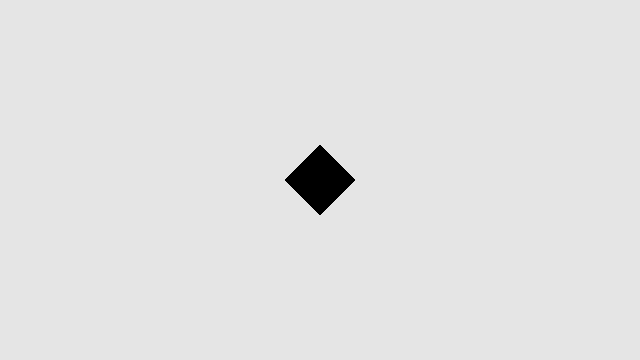
\includegraphics[width=4cm]{images/hello.png}
\end{center}

\subsubsection{GLSL ES}

A GLSL ES nyelv leírása meghaladja ezen jegyzet kereteit.
A nyelv egy rövid kivonata a mellékelt \href{run:./glsl.pdf}{GLSL gyorstalpaló}
dokumentumban olvasható.



\subsubsection{Hello, Twigl!}

Az online Shadertoy egy alternativája a Twigl, amit saját gépünkre telepíthetünk és offline futtathatunk.
A Twigl picit más elnevezéseket használ, ez az alább látható.

\glslexample{Ferde négyzetet rajzoló árnyaló (Twigl verzió)}{../00_intro/peldak/00hello_twigl.glsl}
  
A folytatásban a Shadertoy nyelvjárását fogjuk használni. 

\matfeladatok

Első próbálkozásnak kísérletezhetünk különböző színátmenetekkel. Ehhez normalizáljuk 0 és 1 közé
az $x$ koordinátát, majd a képpontok színét adjuk meg ennek függvényeként.

\begin{glsl}{Átmenetek}
float f(float x) { return /*???*/ }
    
void mainImage( out vec4 fragColor, in vec2 fragCoord )
{
  vec2 uv = fragCoord/iResolution.xy;
  vec3 col = vec3(f(uv.x));
  fragColor = vec4(col,1.0);
}
\end{glsl}

Keressünk $f: [0, 1] \mapsto [0,1]$ átmenet függvényeket a következő tulajdonságokkal.
Lehetőleg ne használjunk elágazást (\texttt{if}) csak aritmetikát és függvényeket.

\begin{enumerate}[resume]
  \item $f$ lineáris, $f(0)=0$, $f(1)=1$.
  \item $f$ majdnem mindig 0, kivéve amikor $|x-0.5|$ ,,kicsi''.
  \item $f$ majdnem mindig 0, kivéve amikor $x$ ,,közel'' esik $0.3$ valamelyik egész többszöröséhez.
  \item $f$ ,,simán'' köti össze a $(0,0)$ és $(1,1)$ pontokat, a végpontokban vízszintes az érintője.
  \item Ugyanaz, mint előbb, de $f$-ről azt is megköveteljük, hogy polinomfüggvény legyen. 
\end{enumerate}

A fentebb készített ábrákra tegyük rá az $y=f(x)$ függvény grafikonját is.

\begin{center}
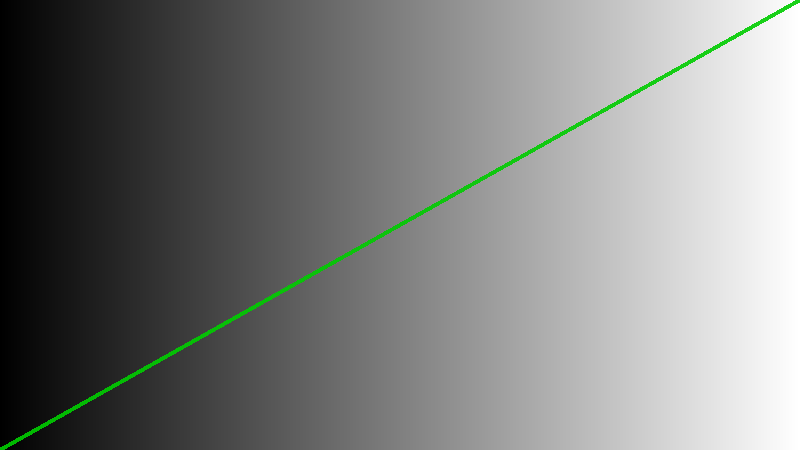
\includegraphics[width=4cm]{images/f01.png}\hfill
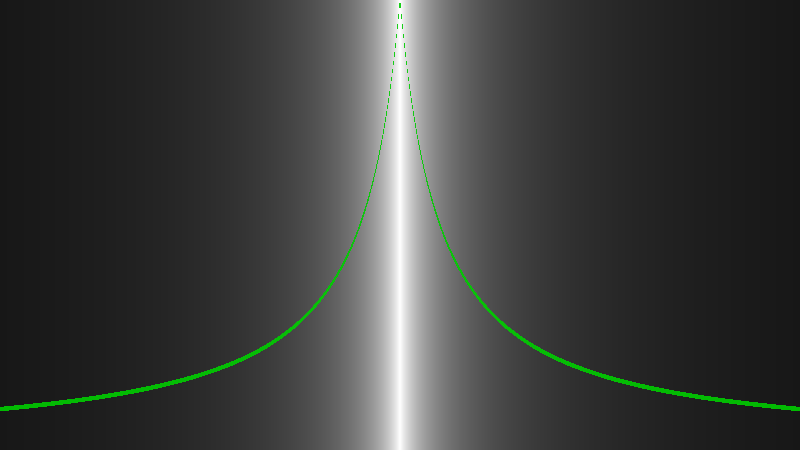
\includegraphics[width=4cm]{images/f02.png}\hfill
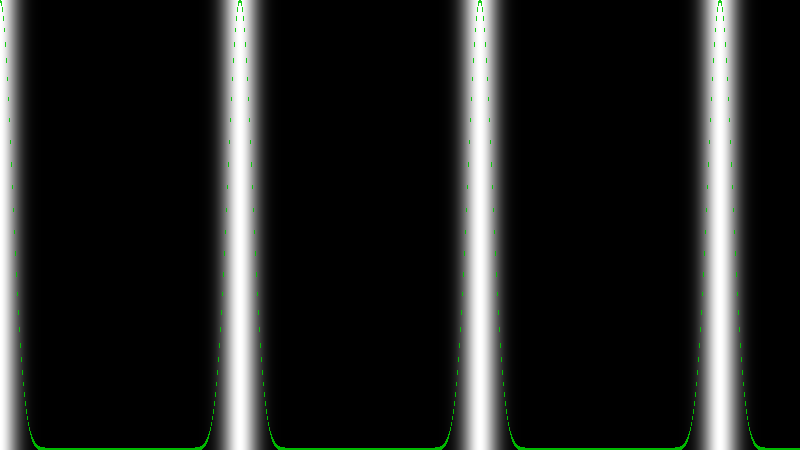
\includegraphics[width=4cm]{images/f03.png}\hfill
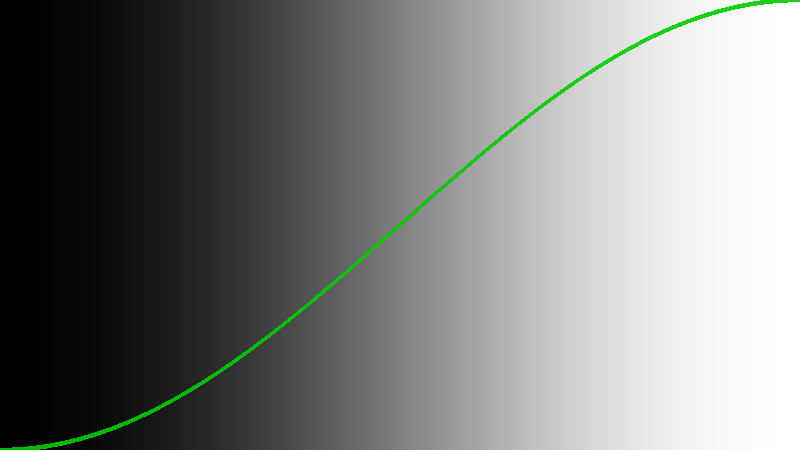
\includegraphics[width=4cm]{images/f04.png}
\end{center}

\subsection{Elemi alakzatok}

A legegyszerűbb ,,modellezési'' megközelítés árnyalókkal az, hogy minden bemeneti koordinátára
eldöntjük, az alakzathoz tartozik-e vagy nem (igen / nem), majd ez alapján vagy az
alakzat színét adjuk vissza, vagy a háttér színét.

\begin{tcolorbox}
  
  $$
  \mathcal{S}: \mathbb{R}^2 \mapsto \mathbb{R}^4,\quad
  \mathcal{A}: \mathbb{R}^2 \mapsto \{igaz, hamis\},\quad
  \mathcal{C}: \{igaz, hamis\} \mapsto \mathbb{R}^4
  $$
  $$\mathcal{S}(x, y) = \mathcal{C}(\mathcal{A}(x,y))$$

  $$\mathcal{A}(x,y) = 
    \begin{cases}
      igaz,  &\text{ha~} (x, y) \text{~az alakzat pontja}\cr
      hamis, &\text{különben}
    \end{cases}
  $$

  $$\mathcal{C}(l) = 
    \begin{cases}
      \text{alakzat szín},  &\text{ha~} l\cr
      \text{háttér szín}, &\text{különben}
    \end{cases}
  $$

  \end{tcolorbox}

\progfeladatok

\begin{enumerate}[resume]
  \item Rajzoljunk adott sugarú kört origó középponttal.
  \item Rajzoljunk adott méretű négyzetet origó középponttal.
  \item Rajzoljunk adott méretű téglalapot adott középponttal.
  \item Rajzoljunk négyzetrácsot.
  \item Színezzük ki a képet sakktábla-szerűen.
  \item Rajzoljunk szabályos háromszöget, amelynek egyik csúcsa az origó.
  \item (*) Rajzoljunk origó középpontú szabályos sokszöget.
\end{enumerate}

\begin{center}
  
\includegraphics[width=2.5cm]{images/f06.png}\hfill
  
\includegraphics[width=2.5cm]{images/f07.png}\hfill
  
\includegraphics[width=2.5cm]{images/f08.png}\hfill
  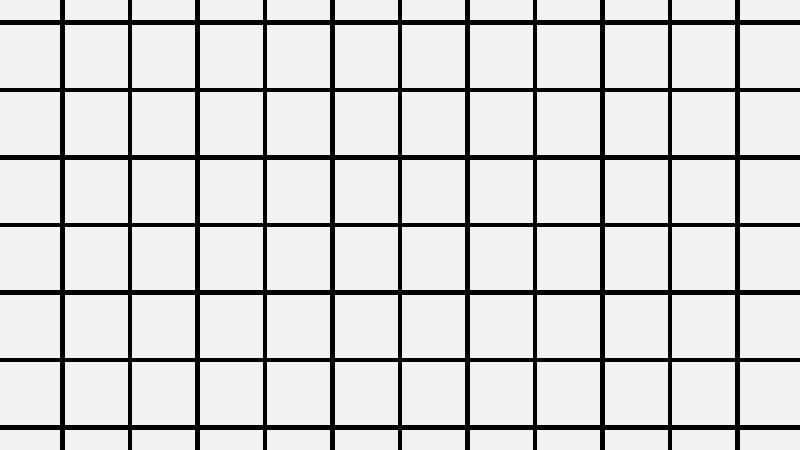
\includegraphics[width=2.5cm]{images/f09.png}\hfill
  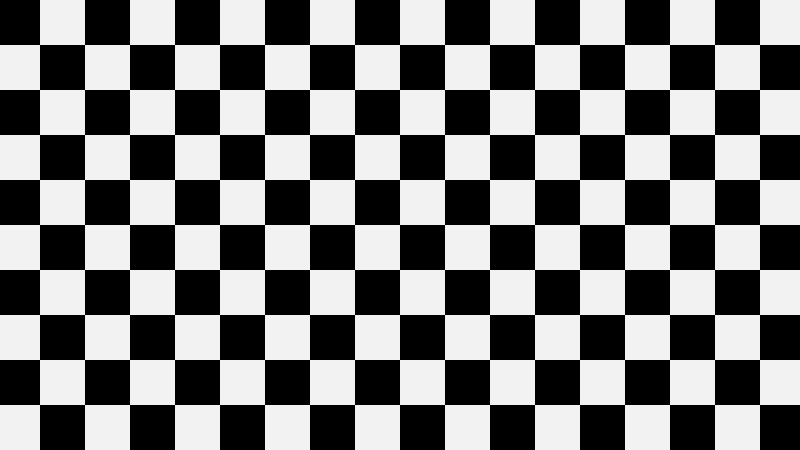
\includegraphics[width=2.5cm]{images/f10.png}\hfill
  
\includegraphics[width=2.5cm]{images/f11.png}\hfill
  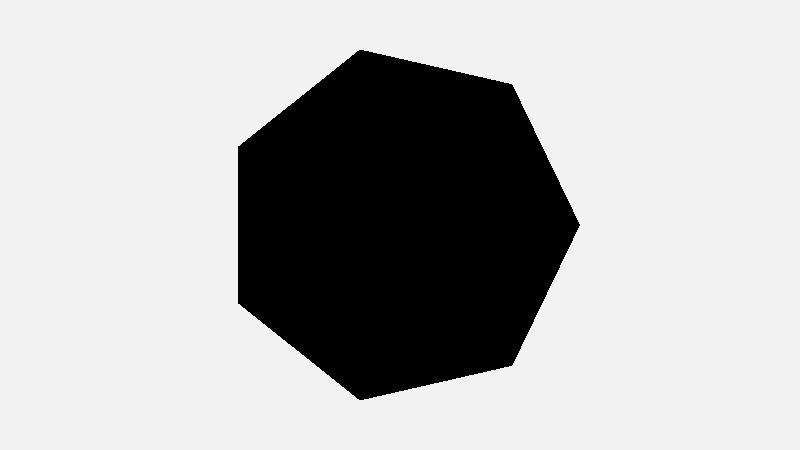
\includegraphics[width=2.5cm]{images/f12.png}
\end{center}

\subsection{Polár-koordináták}

Az \texttt{atan} függvény segítségével egyszerűen átalakíthatunk egy Descartes-koordinátákkal adott
pontot polárkoordinátás alakba:

\begin{glsl}{Polárkoordináták}
float r = length(p);
float alpha = atan(p.y, p.x);
\end{glsl}

Az \texttt{atan} függvény $-\pi$ és $\pi$ közé eső értéket ad, a 0 az X tengely pozitív irányának felel meg.
Szürke árnyalatokkal illusztrálva ($-\pi$ a fekete, $\pi$ a fehér árnyalat):

\begin{center}
  
\includegraphics[width=5cm]{images/atan.png}  
\end{center}

\progfeladatok

\begin{enumerate}[resume]
  \item Rajzoljunk ,,napot'' adott számú ,,napsugárral''.
  \item Rajzoljunk szabályos háromszöget, mint ,,változó sugarú kört''.
\end{enumerate}

\begin{center}
  \hfill
  
\includegraphics[width=4cm]{images/f13.png}\hfill
  
\includegraphics[width=4cm]{images/f14.png}\hfill~
\end{center}

\subsection{Transzformációk és animáció}

\subsubsection{Geometriai transzformációk}

Egy $g$ síkbeli geometriai transzformáció a sík minden pontjához a sík valamelyik pontját rendeli.

$$g(x, y) = (x', y')$$

\matfeladatok

\begin{enumerate}[resume]
  \item Adott egy síkbeli $\mathcal{A}$ alakzat az $\mathcal{S}()$ árnyalóval leírva. Hogyan állítható elő
  az $\mathcal{A}' = g(\mathcal{A})$ alakzat árnyalója?
  \item Adjuk meg a következő transzformációkat formulával:
  (a) eltolás adott vektorral;
  (b) origó körüli, adott szögű forgatás;
  (c) origó középpontú, adott arányú nagyítás;
  (d) origó középpontú, adott sugarú inverzió.
\end{enumerate}

\begin{center}
  \hfill
  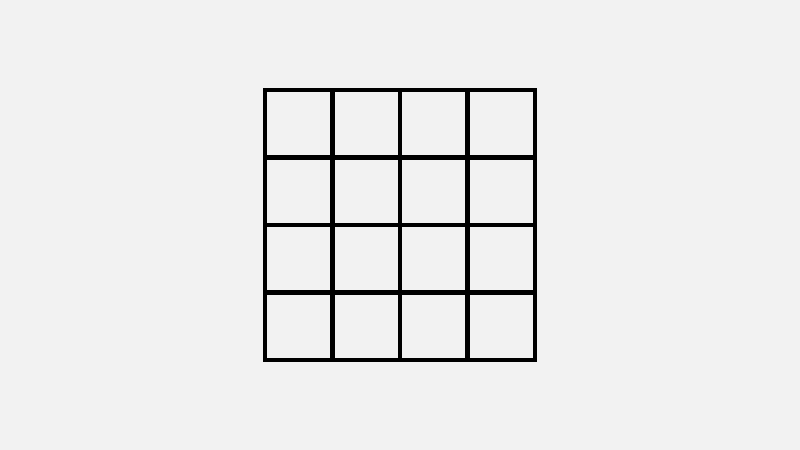
\includegraphics[width=3cm]{images/f16_base.png}\hfill
  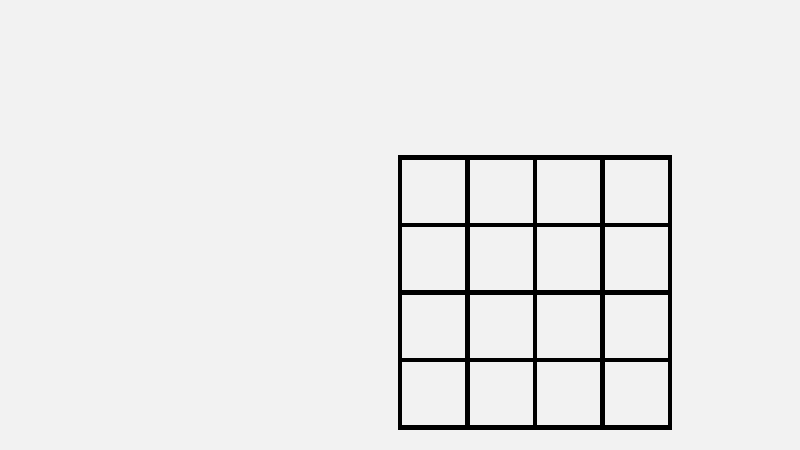
\includegraphics[width=3cm]{images/f16_a.png}\hfill
  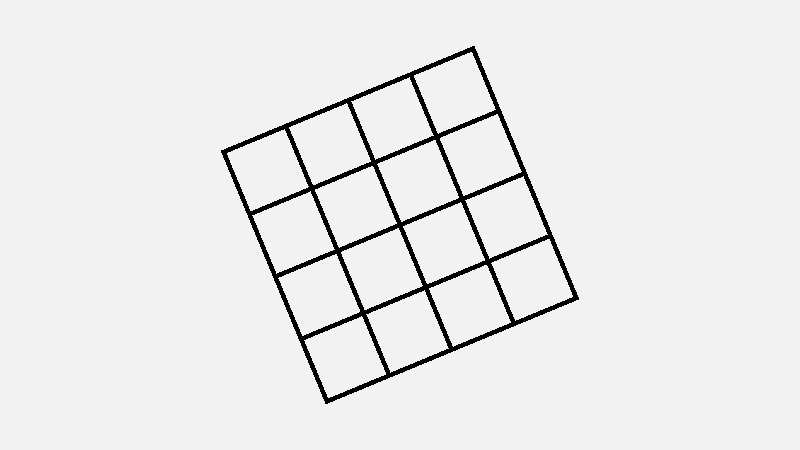
\includegraphics[width=3cm]{images/f16_b.png}\hfill
  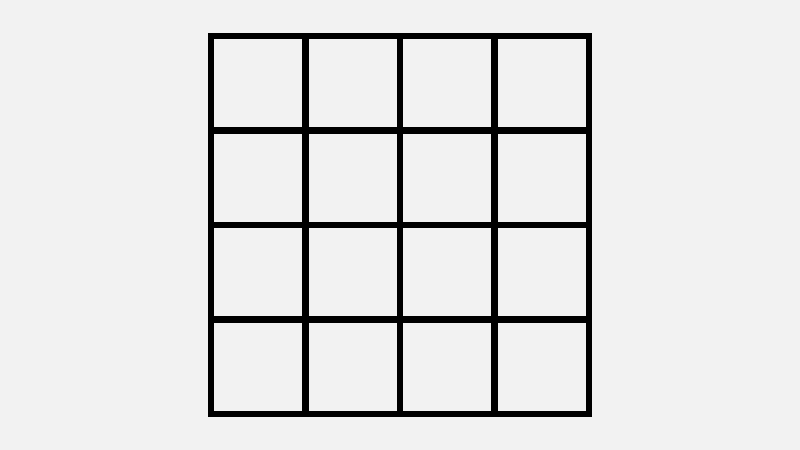
\includegraphics[width=3cm]{images/f16_c.png}\hfill
  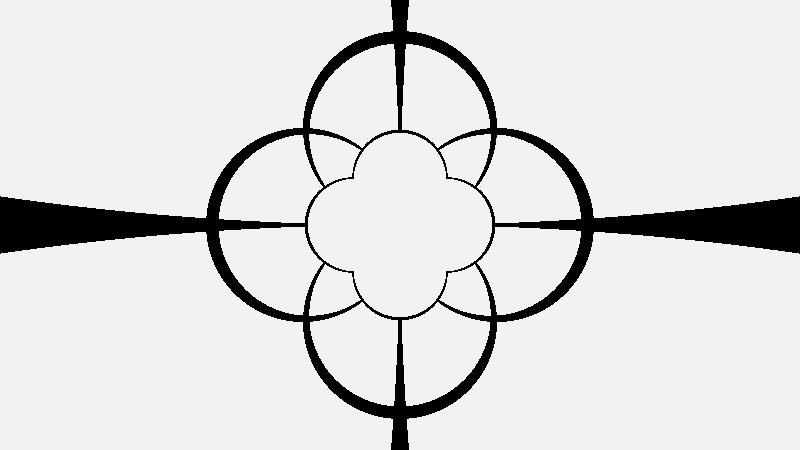
\includegraphics[width=3cm]{images/f16_d.png}\hfill~
\end{center}

\subsubsection{Animációk}
Az árnyékolók nagyon egyszerűen használhatók animációk programozására, csupán
be kell vezetnünk egy idő input változót:

$$\mathcal{S}(x, y, t) = (r, g, b, a)$$

A Shadertoy esetében ez az input változó az \texttt{iTime}, ami másodpercben méri az animáció indítása
óta eltelt időt. Egy képkocka kiszámítása közben minden árnyaló hívás azonos $t$ értéket kap.

Az alábbi példában a kirajzolt kör középpontja
az eltelt időtől függően változik.

\glslexample{,,Pattogó'' labda}{../00_intro/peldak/90bouncingb.glsl}

\progfeladatok

\begin{enumerate}[resume]
  \item Rajzoljunk sakktáblát és forgassuk meg.
  \item Jelenítsünk meg egy szinusz-hullámot periodikusan bejáró kis kört.
\end{enumerate}

\subsection{Iteráció és rekurzió}

Egy egyszerű alakzat fraktál változatát ki tudjuk rajzolni, ha a bemeneti $(x,y)$
ponton több lépésben transzformációkat végzünk.

\progfeladatok
\begin{enumerate}[resume]
  \item Rajzoljunk kis köröket egy $5\times 3$-as rács elrendezésben.
  \item Rajzoljunk Sierpinski-szőnyeget.
  \item Rajzoljunk Sierpinski-háromszöget.
\end{enumerate}

\begin{center}
  \hfill
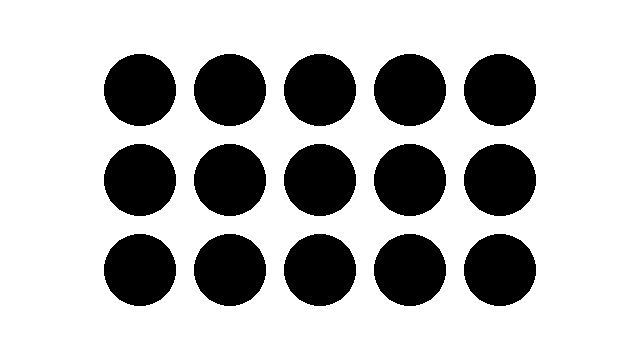
\includegraphics[width=5cm]{images/iter01.png}\hfill
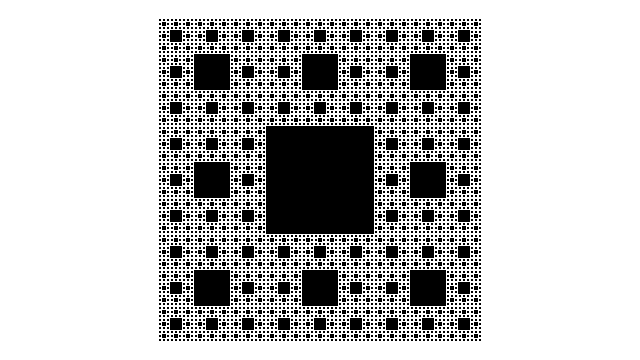
\includegraphics[width=5cm]{images/sier4.png}\hfill
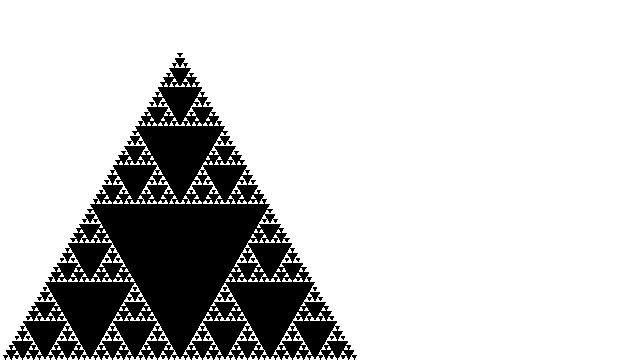
\includegraphics[width=5cm]{images/sier3.png}\hfill~
\end{center}


\section{Előjeles távolság függvények a síkon}

\subsection{Alapok}

\begin{tcolorbox}[title=Előjeles távolság függvény (signed distance function)]
  Az \emph{előjeles távolság függvény} egy $(x,y)$ pont előjeles távolságát adha meg egy ponthalmaz határától mérve.
  Az egyszerűség kedvéért feltehetjük, hogy az alakzat egy zárt, folytonos, nem önmetsző görbével van megadva.
  $$ t: \mathbb{R}^2 \mapsto \mathbb{R}$$
  $$ t(x, y) = d$$

  Ha $(x,y)$ rajta van az alakzat határán, akkor $t = 0$. Külső pontokra $t$ a pont és az alakzat távolságát adja meg.
  Belső pontokra $t$ negatív előjellel adja meg a pont és a határgörbe távolságát.
  
  Az előjeles távolság függvények meglepően jól használhatók arra, hogy egy képet vagy animációt felépítsünk egyszerű
  alap-alakzatokból.
  \end{tcolorbox}

\matfeladatok


Adjuk meg a következő alakzatok előjeles távolság függvényét:

\begin{enumerate}[resume]
  \item Origó középpontú, $r$ sugarú kör.
  \item Origó középpontú, adott méretű, tengely-párhuzamos téglalap.
  \item Végpontjaival adott szakasz.
  \item (*) Szabályos sokszög.
\end{enumerate}

\begin{center}
  \hfill
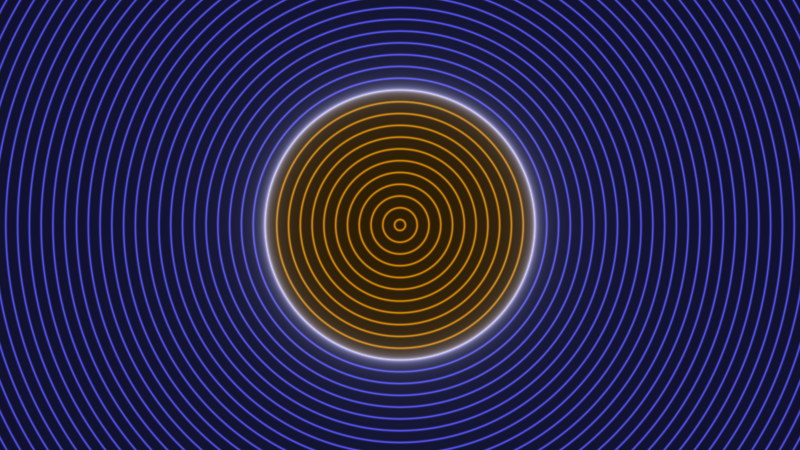
\includegraphics[width=4cm]{images/f22.png}\hfill
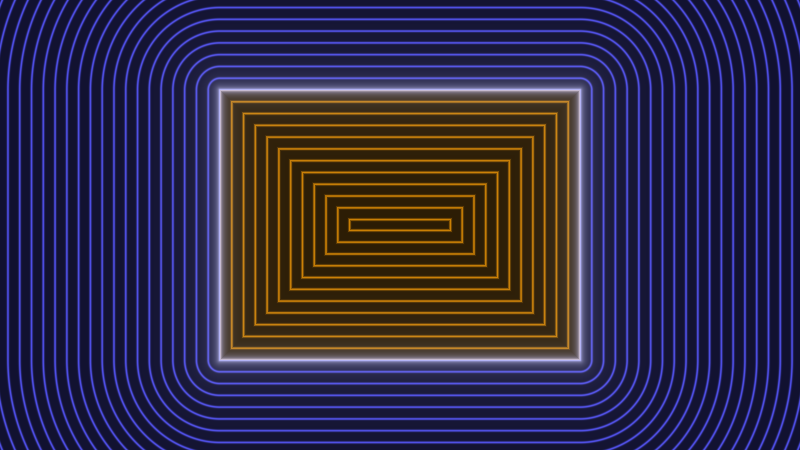
\includegraphics[width=4cm]{images/f23.png}\hfill

\includegraphics[width=4cm]{images/f24.png}\hfill
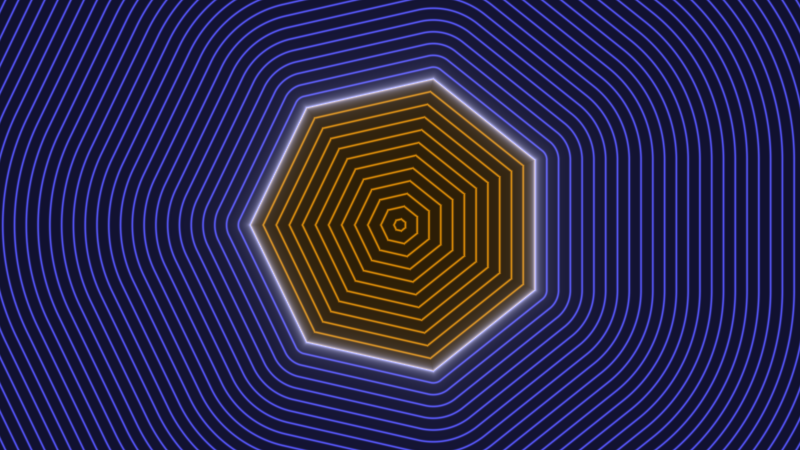
\includegraphics[width=4cm]{images/f25.png}\hfill~
\end{center}

\subsection{Kompozíció és deformáció}

\matfeladatok

\begin{enumerate}[resume]

\item Adott két távolságfüggvénnyel definiált alakzat. Keressünk formulát a
két alakzat
(a) uniójának,
(b) metszetének,
(c) különbségének megjelenítéséhez. A kapott formulák között melyek azok, amelyek
az új alakzat (pontos) előjeles távolságfüggvényét írják le?

\item Hogyan kerekíthető le egy alakzat?

\item Hogyan adható meg egy alakzat (valamilyen vastag) peremének távolságfüggvénye?
\end{enumerate}

\begin{center}
  \hfill
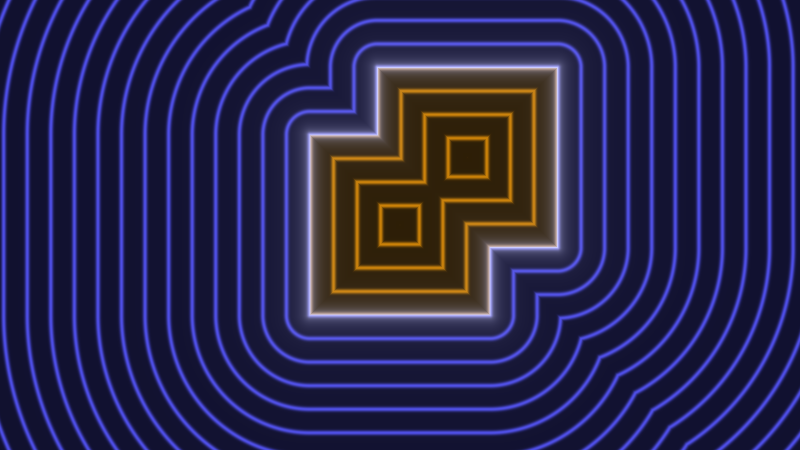
\includegraphics[width=4cm]{images/f26_a.png}\hfill

\includegraphics[width=4cm]{images/f26_aa.png}\hfill

\includegraphics[width=4cm]{images/f26_b.png}\hfill
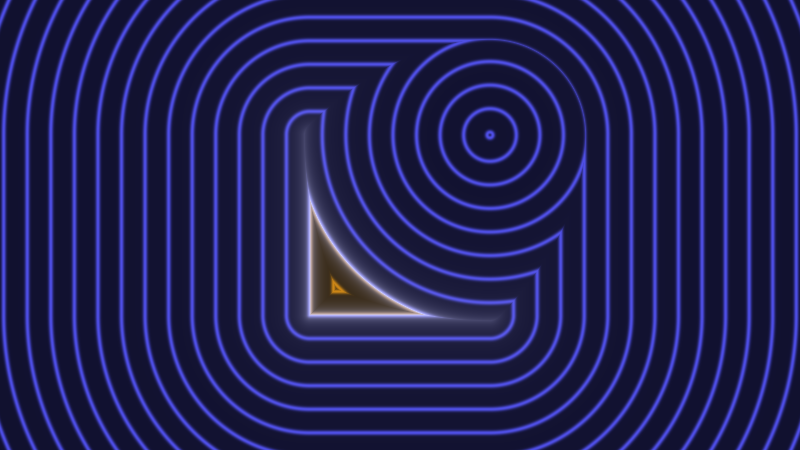
\includegraphics[width=4cm]{images/f26_c.png}\hfill~
\end{center}

\section{Előjeles távolság függvények a térben}

A távolság függvények jól használhatók arra, hogy 3D jeleneteket ábrázoljunk valós időben.
Ehhez a legtöbb 3D modellezési rendszerben a következőkre van szükség:
\begin{description}
  \item[3D modell] Mi ezt most (közelítő) előjeles távolság függvénnyel írjuk le.
  A függvény \emph{világ koordinátákat} (VKR) használ, nem vesz tudomást arról, honnan nézünk rá.
  \item[Kamera] A kamera állapotát két paraméter írja le, a VKR-beli pozíciója és iránya.
  A megjelenítő algoritmusok a 2D kép felbontásától függően a kamera állapotáthoz véges sok félegyenest
  (sugár, ,,ray'') rendelnek és minden sugár egy képpont színének kiszámításáért felel.
  Az alábbi kódokban a sugarak közös kezdőpontja (ami egyben a kamera pozíciója) \texttt{ro} (,,ray origin'')
  és a a sugarak iránya \texttt{rd} (,,ray direction''). Úgy képzelhetjük, hogy a kamera
  iránya a megjeenített téglalap középpontjába mutat.
  \item[Fényforrás(ok)] Ahhoz, hogy lássunk valamit a képen, szükség van legalább egy fényforrásra. Ez
  legegyszerűbb esetben pontszerű, VR-beli pozíciója, színe és intenzitása írja le. Amikor a megjelenítő algoritmus
  azt kapja, hogy egy sugár ,,eltalálta'' a modellt, akkor a képpont színét a találati pont kis környezetéből
  és a fényforrásokból számolja ki.
\end{description} 

\subsection{Sugár séta algoritmus (ray marching)}

A folytatásban, az egyszerűség kedvéért csak homogén anyagokat modellezünk, ezért a sugár séta
algoritmusunk egyetlen számot ad vissza (\texttt{depth}), a találati pont kamerától való távolságát.
Ha ez nagyobb, mint egy rögzített korlát, akkor már túl messze lenne a pont, ezt úgy kezeljük,
hogy az adott sugár nem találta el a modellt. Ilyenkor a képpont valamilyen háttér színt kap (,,fal'', ,,ég'', ...).

A sugár séta algoritmus a kamera pozíciójából indul, az aktuális sugár irányában. Minden lépésben ,,lekérdezi''
a távolság függvényt, és annyit lép előre. Ha a kerekítési hibáktól eltekintünk, akkor nem fordulhat elő,
hogy az objektum belsejébe érünk. Ha egy előre megadott kis értéknél közelebb jutunk az objektumhoz,
akkor úgy tekintjük, hogya sugár eltalálta az objektumot, és visszaadjuk a kamerától való távolságot.
Ha egy rögzített nagy távolságnál messzeb jutottunk, akkor úgy tekintjük, hogy már nem fogjuk eltalálni
az objektumot. 

\glslexample{Egyszerű sugár séta algoritmus}{../02_3d/peldak/raymarching.glsl}

\subsection{Felület normálvektora}

Az előjeles távolság függvénnyel leírt felületün matematikailag egy $f(x, y, z)=0$ egyenlettel
adott \emph{implicit} felület. A többváltozós analízisből tudható, hogy az így leírt felületek
normálvektora (a felületre merőleges, ,,kifelé'' mutató vektor) nem más, mint az $f$ függvény
gradiense az adott pontban.
$$
\nabla f(x, y, z) =
\left(
  \frac{\partial f}{\partial x}, 
  \frac{\partial f}{\partial y}, 
  \frac{\partial f}{\partial z} 
\right)
$$
A gradiens vektor koordinátáit közelíthetjük az előjeles távolság függvényből számított
szimmetrikus differenciák segítségével. Itt motivációként gondolhatunk az egyváltozós függvények esetében
ismert Lagrange-féle középérték tételre: 
$f'(x_0)\approx \frac{f(x_0+\epsilon) - f(x_0-\epsilon)}{2\epsilon}$.

\glslexample{Normálvektor számítása (közelítő)}{../02_3d/peldak/surface_normal.glsl}

Érdemes megjegyezni, hogy ez a számítás nagyon érzékeny $\epsilon$ értékére és arra is, hogy a
távolság függvényünk mennyire pontos. (A tipikus kompozíciók általában ,,elrontják'' a távolság függvényt, 
de szerencsére sok esetben a felülethet ,,közel'' ez a hiba még elhanyagolható.)

\subsection{Phong megvilágítási modell}

A Phong megvilágítási modell egy jelentősen leegyszerűsített képlet felületi pontok
színezéséhez. Három komponensből számítja ki egy pont színét.

\begin{description}
  \item[háttér, ambient] Ez a színtér minden pontjában konstans. Például egy kékre festett szobában
  minden pont egy kicsit kék, ha nincs teljesen sötét.
  \item[szórt, diffuse] A felületi pontból minden irányba azonos intenzitással visszavert fény. Az
  intenzitás a beeső fénysugár irányának és a felület normálvektorának szögétől függ,
  akkor maximális, amikor a fénysugár a felületre merőlegesen érkezik.
  \item[tükröződő, specular] A visszavert fény intenzitása attől függ, mekkora szöget zár be
  a beeső fénysugár tükörképe a kamera irányával. Ha olyan irányból nézünk a felületre, amerre
  a tükrözött fénysugár tart, akkor csillogónak látjuk az objektumot.
\end{description}

\begin{center}
  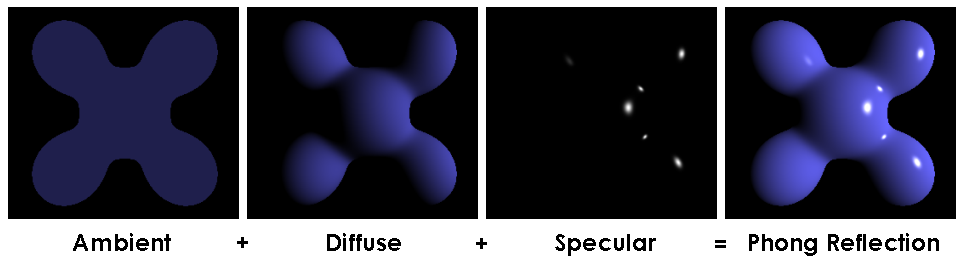
\includegraphics[width=15cm]{images/phong.png}
\end{center}
  

\glslexample{Phong megvilágítási modell}{../02_3d/peldak/phong.glsl}

A példában a számított szín koordinátáit még kicsit módosítjuk a végén (gamma-korrekció).
Az elvégzett hatványozás nagyjából egy gyökvonásnak felel meg, ami azt eredményezi, hogy
a sötétebb tartományokban ,,széthúzzuk'', a világos tartományokban ,,összenyomjuk''
a színeket. Erre azért van szükség, mert az emberi szem máshogy ,,méri'' az intenzitást, mint
a digitális kamerák. 

\subsection{Kamera animáció}

OpenGL konvenció, hogy pozitív körüljárású koordinátarendszert használunk és a $Z$ tengely
a színtér felől a kamera felé mutat.
(\url{https://learnopengl.com/Getting-started/Camera})

\begin{center}
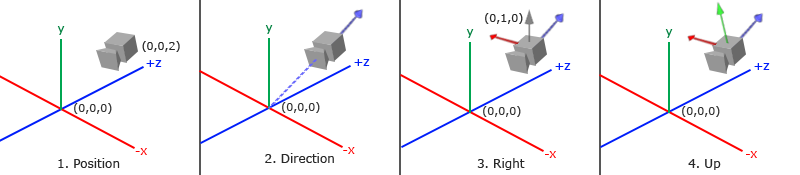
\includegraphics[width=16cm]{images/camera_axes.png}
\end{center}

\glslexample{Adott pontból adott pont felé néző kamera}{../02_3d/peldak/camera.glsl}

Az egér pozícióját változtatva forgathatjuk a kamerát egy rögzített pont körül,
és az előző függvény segítségével elérhetjök, hogy mindig egy rögzített pont felé nézzen.

\glslexample{Példa: forgatható kamera az árnyalóban}{../02_3d/peldak/ray.glsl}

\subsection{Sima kompozíció}

Amikor elemi alakzatok uniójaként állítunk elő komplexebb alakzatokat, előfordul, hogy
szeretnénk elkerülni az ,,éles'' metszésvonalakat és azt várjuk, hogy a két elemi alakzat
,,olvadjon egymásba'' (blending). Ennek matematikai eszköze a ,,sima minimum'' (smooth min),
aminek lényege, hogy ha két érték különbsége egy adott korlátnál kisebb, akkor minimumuk helyett
valamilyen kombinációjukkal számolunk.

\begin{glsl}{Példa: polinomilális sima minimum (k=.2))}
float smin( float a, float b, float k )
{
  float h = clamp( 0.5 + 0.5 * (b - a) / k, 0.0, 1.0 );
  return mix( b, a, h ) - k * h * (1.0 - h);
}
\end{glsl}


\begin{center}
  \hfill
  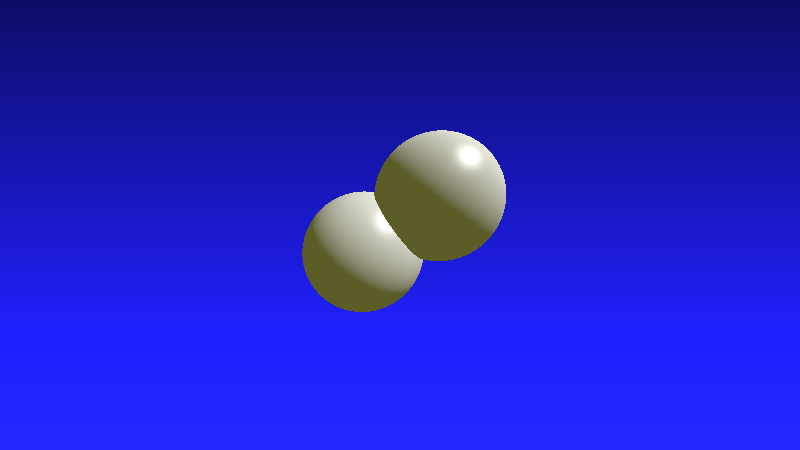
\includegraphics[width=5cm]{images/uni-min.png}\hfill
  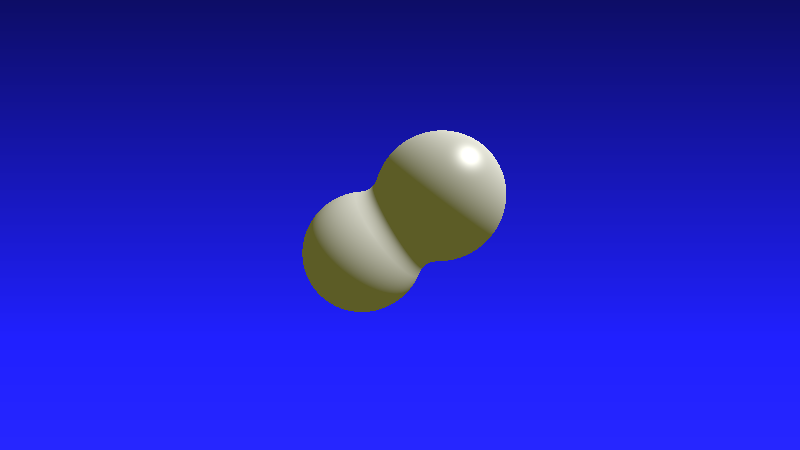
\includegraphics[width=5cm]{images/uni-smin.png}\hfill~
  \end{center}

\subsection{Teljes példa}

Zárszóként egy térbeli szakaszok megvastagításával kapott kapszulákból
összeállított 3D szöveg teljes kódját közöljük.


\begin{center}
  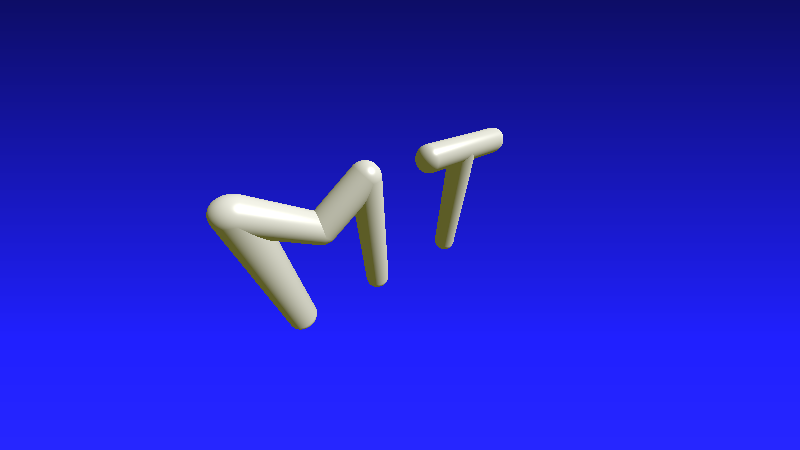
\includegraphics[width=8cm]{images/final.png}
  \end{center}

\glslexample{3D szöveg szakaszokból}{../02_3d/peldak/final_scene.glsl}


\glslexample{Szöveg forgatása}{../02_3d/peldak/final_anim.glsl}

\end{document}
